\documentclass[conference]{IEEEtran}
\IEEEoverridecommandlockouts

\usepackage{cite}
\usepackage{amsmath,amssymb,amsfonts}
\usepackage{algorithmic}
\usepackage{graphicx}
\usepackage{multirow}
\usepackage{textcomp}
\usepackage{xcolor}
\usepackage{subfigure}
\usepackage[brazil]{babel}



\begin{document}



\title{Comparação entre os métodos \textit{grid} e \textit{quadtree} para compressão de dados em aplicações \textit{online}}

\author{
\IEEEauthorblockN{Rafael Fernandes Gonçalves da Silva}
\IEEEauthorblockA{\textit{Departamento de Engenharia Elétrica} \\
\textit{Universidade Federal de Minas Gerais}\\
Belo Horizonte, Brasil \\
rafaelfgs@ufmg.br}
}

\maketitle

\begin{abstract}
Este trabalho consiste na utilização de métodos baseados em \textit{grid} e \textit{quadtree} para redução na amostragem e com algumas modificações de forma a tornar-se incremental. A aplicação de ambos os métodos gera uma superfície de densidade, sendo fixa para \textit{grid} e variável para o \textit{quadtree}. A avalição dos métodos é realizada através dos valores da acurácia e da economia de alocação de memória, esta representada pela quantidade de espaços utilizados na superfície. Em ambos os métodos é feita uma combinação entre a superfície criada no pacote anterior e no atual, utilizando um fator de esquecimento para dar um peso maior nos dados antigos ou nos atuais. Os testes são feitos principalmente na base de dados disponibilizada \textit{SyntheticDatasetRodrigo}. Por fim, são utilizados outras duas base de dados: \textit{sea} e \textit{fourclass}, onde é possível observar as propriedades do \textit{grid} e do \textit{quadtree} através de outros métodos de entradas de dados.
\end{abstract}

\global\long\def\IEEEkeywordsname{Palavras-chave}
\begin{IEEEkeywords}
Classificação \textit{online}, \textit{grid}, \textit{quadtree}
\end{IEEEkeywords}



\section{Introdução} \label{intro}

Os métodos incrementais de classificação estão se tornando cada vez mais importantes nos dias atuais. O avanço tecnológico provocou um aumento gigantesco na criação e na utilização de informações envolvendo diversos campos distintos, como economia, telecomunicações, plataformas sociais, indústrias das mais diversas formas, entre outros. Em muitos desses campos, a informação necessita ser tratada em tempo real, já que o acesso à sua totalidade pode não estar disponível, com os dados sendo recebidos em formas de pacotes, e ainda podem ocorrer mudanças de comportamento dos dados ao longo do tempo.

Classificadores em tempo real são bastante comuns, sendo amplamente utilizados na área de visual computacional. Os trabalhos propostos em \cite{castro2018end}, \cite{shrivastava2016training} e \cite{hong2015online} utilizam redes neurais convolucionais e algoritmos de forma \textit{online} para classificar e reconhecer objetos à medida em que chegam os dados. Especificamente, conforme citado em \cite{castro2018end}, o reconhecimento de faces em tempo real torna-se mais interessante, onde uma nova face de entrada não acarreta uma total reclassificação dos dados antigos.

A classificação de forma \textit{online} pode ser aplicada em dados relacionados à internet, como em \cite{mohammed2009near} e \textit{ibrahim2016internet}, onde são utilizados algoritmos de aprendizado de máquina para detectar e classificar tráfego de internet. Pode ser também aplicada no reconhecimentos de palavras em textos e/ou documentos para identificar e adaptar perfis de usuário em tempo real, conforme explicado em \cite{bouchachia2014online}, ou para reconhecer situações de emergência em mensagens de usuários em mídias sociais, como explicado em \cite{yin2015using}.

Há também aplicações para a área financeira, onde \cite{cao2019titant} e \cite{patel2019application} utiliza métodos de classificação em tempo real para detectar fraudes em transações financeiras e manipulações de relatórios para ocultações de perdas financeiras.

Os métodos de classificação incremental mais comuns necessitam de uma memória representativa dos dados, visto que o armazenamento de dados no seu formato original em um sistema contínuo por longos períodos de tempo torna-se inviável. Além disso, pode haver mudanças de conceito, onde o armazenamento de dados antigos passa a ser desnecessário após um tempo. Dessa forma, a compressão e representação de dados torna-se importante no contexto de classificação de grandes bases de dados e de métodos incrementais.

Há vários métodos para a realização da compressão de dados. Em \cite{wlodarczyk2017fragmentation}, é realizada uma fragmentação de dados hidrográficos em subconjuntos na forma de \textit{grids}, resultando em uma subamostragem. A redução do consumo de memória pode ser feita também através de grids hexagonais, como realizado em \cite{knaup2007ct} utilizando diferentes dados de sinais e imagens. O método de \textit{quadtree} é utilizado em \cite{basilico2012online} para a realização de representações espaciais de imagens tomadas por utilizando Veículos Aéreos Não-Tripulados durante um patrulhamento. Pode-se também realizar uma comparação entre os diferentes métodos, como é feito em \cite{beltrami2015grid}, onde são realizados e comparados métodos de busca de hiper-parâmetros de um \textit{Support Vector Machine} através de \textit{gridsearch} e \textit{quadtree}, ou como em \cite{wai2018comparison}, onde são comparadas as perdas de compressão dos métodos \textit{block-encoding} e \textit{octree} utilizando imagens de mapas como bases de dados.

Partindo dessas contextualizações, o presente trabalho tem por objetivo a comparação de dois métodos de compressão de dados: \textit{grid} e \textit{quadtree}, implementados de forma a funcionar para um fluxo de dados. São utilizadas três base de dados: \textit{SyntheticDatasetRodrigo.csv}, \textit{sea.data} e \textit{fourclass}, sendo as duas primeiras disponibilizadas previamente e a última disponível no pacote \textit{Evidential Clustering} (\textit{evclust}) do repositório \textit{CRAN} para a linguagem R. O código foi criado utilizando a base de dados \textit{SyntheticDatasetRodrigo}, onde foi observado o seu comportamento para uma dada variação dos parâmetros de entrada.



\section{Metodologia} \label{metod}

De uma forma bastante resumida, a metodologia utilizada consiste em comprimir uma base de dados para um formato de \textit{grid} e um de \textit{quadtree}, gerando uma probabilidade para cada intervalo dos formatos e partir disso criar um modelo de classificação.

O código implementado foi separado em quatro partes, descritas nas subseções seguintes.



\subsection{Entradas do Algoritmo} \label{metod_1}

A leitura da base de dados é o primeiro passo realizado pelo algoritmo. Para ficar de forma padronizada, a base de dados deve estar no formato matricial com três colunas e $n$ linhas, onde as colunas representam a primeira variável, a segunda variável e os rótulos e as linhas representam as amostras. A base de dados \textit{sea} possui três variáveis e teve de ser dividida em três bases de dados de forma a ser aplicada em pares de variáveis: 1 com 2, 1 com 3 e 2 com 3.

Em seguida são determinadas as constantes globais do algoritmo, sendo um total de quatro: \textit{forg\_factor} representa o fator de esquecimento, ligado à relação entre as antigas e novas representações dos dados; \textit{batch\_size} corresponde ao tamanho do pacote de entrada dos dados, nesse caso a base de dados foi dividida em pacotes de tamanhos iguais; \textit{num\_parts} está relacionado ao número de divisões do espaço, onde o espaço é divido em \textit{num\_parts} x \textit{num\_parts} para o \textit{grid} e o número de levels do \textit{quadtree} é dado por $\left \lfloor log_{2}(num\_parts) \right \rfloor+1$; e \textit{apply\_filt} indica se será realizada ou não a filtragem para o método do \textit{grid}, sendo esta uma constante binária.

\begin{figure}[h]
\centerline{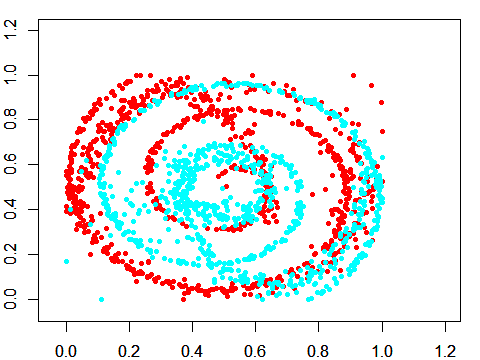
\includegraphics[width=0.55\columnwidth]{fig/rodrigo.png}}
\caption{Amostras da base de dados \textit{SyntheticDatasetRodrigo}.}
\label{rodrigo}
\end{figure}

\begin{figure}[h]
\centerline{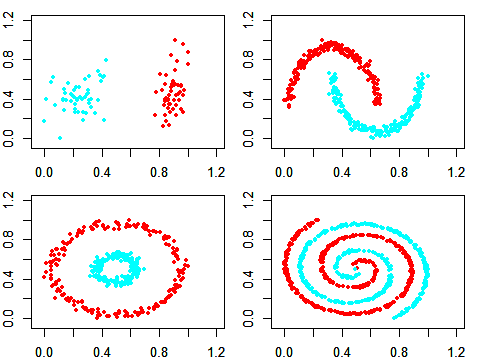
\includegraphics[width=0.6\columnwidth]{fig/rodrigo_parts.png}}
\caption{Amostras da base de dados disponibilizada dividida em cada conceito. A ordem temporal dos dados ocorre primeiramente acima da esquerda para a direita.}
\label{rodrigo_parts}
\end{figure}

\begin{figure}[h]
\centerline{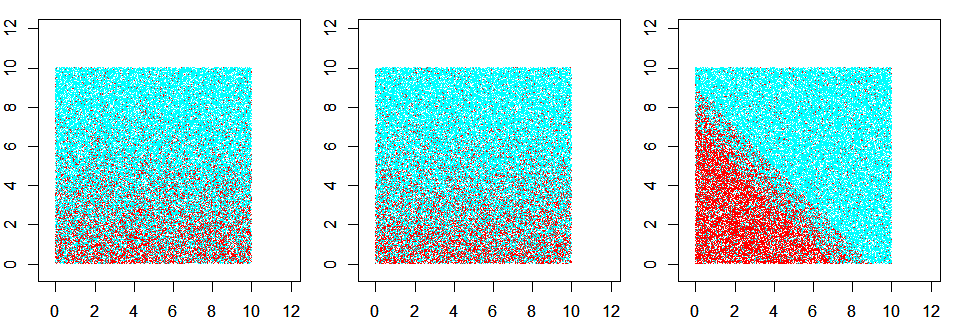
\includegraphics[width=1\columnwidth]{fig/sea.png}}
\caption{Amostras da base de dados \textit{sea}. Da direita para a esquerda estão representadas as variáveis 1 e 2, 1 e 3, 2 e 3.}
\label{sea}
\end{figure}

\begin{figure}[h]
\centerline{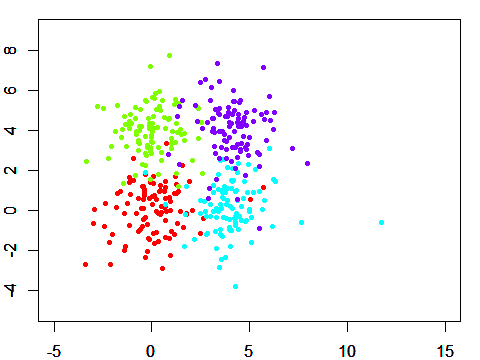
\includegraphics[width=0.6\columnwidth]{fig/four.png}}
\caption{Amostras da base de dados \textit{fourclass}.}
\label{four}
\end{figure}

As bases de dados utilizadas estão representadas nas Figuras \ref{rodrigo}, \ref{sea} e \ref{four}, sendo esta segunda dividida em pares de variáveis. A Figura \ref{rodrigo_parts} mostra as mudanças de conceito da base de dados, onde os primeiros 100 dados são gaussianas separáveis, do 101 ao 500 são duas parábolas invertidas, do 501 ao 900 são dois círculos concêntricos e do 901 ao 1700, duas espirais.



\subsection{Funções Necessárias} \label{metod_2}

Nessa parte do algoritmo encontram-se as funções necessárias para o funcionamento do código. São aqui trabalhadas duas variáveis principais: matrizes de probabilidade e modelo de classificação. A primeira representa as probabilidades de cada classe para um dado intervalo, apresentada na Tabela \ref{pmatrix}. Possui um formato $n$ x $(4+k)$, onde $n$ é o número de intervalos necessários, as quatro primeiras colunas são os valores desses intervalos para as variáveis 1 e 2 e as $k$ próximas colunas são as probabilidades de cada classe (note que $n$ e $k$ podem variar com o tempo). O modelo de classificação é similar à matriz de probabilidades, possui em formato $n$ x $5$, sendo que na quinta coluna estão os rótulos associado à cada intervalo, encontrados através da classe que possui a maior probabilidade naquele intervalo.

\begin{table}[h]
\caption{Matriz de probabilidade para três classes e quatro intervalos.}
\tabcolsep=0.12cm
\begin{center}
\begin{tabular}{ccccccc}
\hline
$x1_{min}$ & $x1_{max}$ & $x2_{min}$ & $x2_{max}$ & $prob_{1}$ & $prob_{2}$ & $prob_{3}$ \\ \hline
0 & 0.5 & 0 & 0.5 & 0      & 0.01 & 0.16 \\
0 & 0.5 & 0.5 & 1 & 0.17 & 0.07 & 0.11 \\
0.5 & 1 & 0 & 0.5 & 0.18 & 0.05 & 0      \\
0.5 & 1 & 0.5 & 1 & 0.05 & 0.18 & 0.05 \\ \hline
\end{tabular}
\label{pmatrix}
\end{center}
\end{table}

\subsubsection{\textit{createGrid}} \label{metod_21}

Função utilizada para criar e combinar duas matrizes dados para o método \textit{grid}. Possui sete parâmetros de entrada: os vetores das variáveis 1 e 2 das amostras da iteração atual, seus respectivos rótulos, as classes até então observadas, a matriz de probabilidade da iteração anterior e os intervalos desejados das variáveis 1 e 2. Inicialmente a matriz antiga de probabilidade é transformada em um grid do tamanho especificado. Em seguida é criado um \textit{grid} com as probabilidades das amostras da iteração atual, essa probabilidade de um intervalo é calculada pela divisão entre do número de amostras do intervalo e número total de amostras. Em seguida é aplicado um filtro de forma a suavizar o \textit{grid} de probabilidades (note que o filtro utilizado está normalizado de forma a não alterar a probabilidade total do \textit{grid}. Em seguida é feita a combinação entre o \textit{grid} antigo com o novo através do fator de esquecimento de forma a ponderar ambos os \textit{grids} sem alterar a probabilidade total. Por fim, o \textit{grid} resultante é transformado em uma matriz probabilidade, a qual representa o retorno da função.

\subsubsection{\textit{combineTree}} \label{metod_22}

Função utilizada para combinar duas matrizes de probabilidade para o método de \textit{quadtree}, visto que o intervalos presentes nas matrizes podem ser diferentes. Para isso, percorre-se as linhas de cada matriz e, quando é encontrado algum intervalo diferente, os valores de probabilidade da matriz com o intervalo maior são distribuídos entre os intervalos menores de forma balanceada. A combinação entre as matrizes agora equivalentes é feita através do fator de esquecimento de forma obter uma ponderação entre a representação antiga e a nova. A função retorna o resultado da combinação.

\subsubsection{\textit{createTree}} \label{metod_23}

Esta função é utilizada para criar as matrizes de probailidade atual para o \textit{quadtree}. Também possui sete parâmetros de entrada, similar a \textit{createGrid}: os vetores das variáveis 1 e 2, os rótulos, as classes, a matriz de probabilidade e os intervalos. Para encontrar os intervalos do \textit{quadtree}, é percorrido o limite máximo de divisões, mas a divisão somente é computada no intervalo em quatro condições: alcançar o limite máximo de divisões, houver apenas amostras de uma classe, não houver nenhuma amostra, ou houver uma classe em todo o espaço. De forma similar a probabilidade de um dado intervalo é o número de amostras nele dividido pelo número total de amostras. Ao final a função \textit{combineTree} é chamada para combinar as matrizes de probabilidade antiga e nova.

\subsubsection{\textit{createModel}} \label{metod_24}

Esta função recebe as matrizes de probabilidade (de qualquer um dos métodos) e, percorrendo cada linha da matriz, determina a classe correspondente ao intervalo através da maior probabilidade entre as classes. A função retorna o modelo de classificação, com os intervalos e a sua respectiva classe.

\subsubsection{\textit{predModel}} \label{metod_25}

Função para determinar as classes das amostras de teste. Possui como entradas os vetores das amostras de teste (variáveis 1 e 2), os valores das classes já observadas e o modelo de classificação. Para determinar a classe de uma amostra, é observado seu respectivo intervalo no modelo de classificação e observado o índice correspondente. A função retorna as predições das amostras, de acordo com os índices e os valores das classes já observadas.

\subsubsection{\textit{plotBase}} \label{metod_26}

Função com propriedades gráficas para exibir a base de dados atual na tela. Possui como entrada a base de dados e os limites das variáveis 1 e 2.

\subsubsection{\textit{plotClassifier}} \label{metod_27}

Função com propriedades gráficas para exibir os resultados obtidos. Foi implementada de forma a exibir em tempo real o modelo do classificador, possuindo como entradas o modelo \textit{grid}, o modelo \textit{quadtree}, as classes e o tipo de exibição, onde valores verdadeiros exibem em tempo real (adicionando uma pausa e limpando o espaço de plotagem) e valores falsos exibem os modelos encontrados em todas as iterações. Para exibir os modelos, estes são transformados em formato de \textit{grid} e mostrados como imagens.



\subsection{Limites da base de dados} \label{metod_3}

Nesta parte do algoritmo é encontrada a melhor forma de representação dos espaços, sendo calculados os limites máximos e mínimos de cada variável e, de acordo com a constante do número de divisões, as sequências dos intervalos do \textit{grid} e do \textit{quadtree}.



\subsection{Classificador Online} \label{metod_4}

Esta representa a parte principal do algoritmo, onde inicia-se as variáveis e chama-se as funções. Foi introduzido o conceito de quantidade de memória utilizada, sendo representada pelo número de intervalos necessários para cada método realizar a classificação. Para o \textit{grid}, essa quantidade é sempre fixo, sendo igual ao quadrado da constante do número de divisões do espaço. Para o \textit{quadtree}, essa quantidade pode variar de acordo com a posição dos dados de entrada.

Depois de iniciadas as variáveis da acurácia e de quantidade de memória, o código entra em um \textit{loop} de acordo com o tamanho da base de dados e a constante global do tamanho dos pacotes de entrada. Primeiramente, são determinados os índices relacionados ao pacote atual, onde são selecionados 70\% para treino do modelo e 30\% para teste. Em seguida, são determinadas as variáveis das classes e das matrizes de probabilidades e, caso o número de classes se alterar, são adicionadas colunas nulas nas matrizes de probabilidades. Por fim, para cada um dos dois métodos, faz-se os seguintes passos: é atualizada a matriz de probabilidades de acordo com os dados de treino e a matriz da iteração anterior, é criado o modelo de classificação utilizando a matriz de probabilidades, são feitas as predições dos dados de teste com o modelo encontrado, é determinada a acurácia e a quantidade de memória utilizada pelo método. Ao final de cada iteração, pode-se exibir o resultado do modelo encontrado em tempo real. Depois de finalizado o \textit{loop}, são exibidos alguns resultados finais.



\section{Resultados e Discussão} \label{result}

Os testes principais para verificar o funcionamento e o desempenho do código foram realizados com a base de dados \textit{SyntheticDatasetRodrigo}. Com essa base, foram realizados diferentes testes avaliando a resposta do código em função de diferentes valores de suas constantes globais. Ao final, o código também foi testado nas bases de dados \textit{sea} e \textit{fourclass}, porém com os parâmetros fixos.

Para a base de dados \textit{SyntheticDatasetRodrigo}, foi estabelecido de forma empírica valores padrão das constantes globais, sendo $\textit{forg\_factor} = 2/3$, $\textit{batch\_size} = 32$, $\textit{num\_parts} = 16$ e $\textit{apply\_filt} = $VERDADEIRO. Os resultados obtidos com a variação desses parâmetros estão representados nas Figuras \ref{accforg}, \ref{accbatch}, \ref{accparts} e \ref{accfilt} e na Tabela \ref{tabon}. Nessa tabela as constantes $k_{1}$, $k_{2}$, $k_{3}$ e $k_{4}$ são representadas pela mesma sequência citada acima.

A utilização de maiores pesos para os novos dados gera uma resposta mais rápida e mais instável tendo melhores resultados para classificações mais simples, porém piores para mais complexas. Enquanto que um peso maior para os dados antigos, reduz o tempo de resposta, porém atinge melhores resultados a longo prazo. Neste cenário, os resultados do \textit{quadtree} foram pouco piores em relação ao \textit{grid}, mas com uma redução de memória maior que 60\%.

A redução do tamanho do pacote também gera uma instabilidade dos modelos, enquanto que pacotes muito grandes não são úteis em ambientes com frequentes mudanças de conceito. Nesse caso o \textit{quadtree} tem uma maior instabilidade e uma maior economia de memória em pacotes pequenos, e, em pacotes maiores, quase se iguala ao \textit{grid}, com uma redução de mais de 50\% de memória.

O aumento do número de divisões do espaço provoca uma melhora dos resultados para o \textit{grid}, juntamente com um aumento exponencial de memória. O \textit{quadtree} mostrou-se indiferente para as variações realizadas, sendo melhor que o \textit{grid} em 8 divisões (com redução de 30\% de memória) e pior em 32 divisões (com redução de mais de 90\%). A Figura \ref{memparts} também demonstra essa redução no gasto de memória.

A aplicação do filtro no \textit{grid} mostrou resultados melhores em classificações mais simples, enquanto que sua retirada provoca resultados melhores a longo prazo. Isso pode ser visto através das Figuras \ref{off} e \ref{offfilt}, onde o modelo perde desempenho para classes muito próximas. Esse fato pode também ser observado na Tabela \ref{taboff}, onde o \textit{grid} sem o filtro obteve resultados similares ao \textit{quadtree}.

Foi também observada a capacidade reativa dos modelos. As Figuras \ref{driftgmodel} e \ref{drifttmodel} demonstram a adaptação do modelo no momento em que ocorre uma mudança de conceito. Pode-se observar que para o \textit{grid} a mudança ocorre de uma forma mais suave e é possível verificar o formato dos dados, enquanto que no \textit{quadtree}, as mudanças ocorrem somente onde é necessário (intervalos onde ocorrem duplicidade de classes diferentes), tornando-se mais econômico porém com uma pior aparência.

Por fim, utilizando as outras bases de dados, através da Tabela \ref{tabsea} e da Figura \ref{seaacc}, pode-se observar a uma grande oscilação (não crescente) no valor da acurácia e uma baixa economia de memória do \textit{quadtree}, demostrando a complexidade de classificação da base \textit{sea} (resultados gerados com as constantes iguais à $2/3$, $128$, $32$ e $1$). Já para a base de dados \textit{fourclass}, onde cada pacote representa uma classe diferente, o \textit{quadtree} obteve um erro quase completo da seguanda classe. Esse fato deve-se à não ocorrência de sobreposições dentro de cada pacote, visto que não houve divisões do espaço fazendo com que os pontos da terceira classe fosse preditos para a primeira classe (resultados gerados para à $2/3$, $100$, $8$ e $1$).



\section{Conclusão} \label{concl}

Através dos resultados obtidos, pode-se concluir que os métodos utilizados podem ser utilizados em um contexto \textit{online} de forma incremental, retendo informação de entradas anteriores e se adaptando a novas distribuições das amostras. Foi possível observar uma grande redução na utilização de memória, principalmente para o método \textit{quadtree}, visto que sua divisão do espaço se adpta ao formato dos dados reduzindo o gasto em regiões de mesma ou com nenhuma classe.

De forma a aprimorar os resultados, são citados algumas possíveis atualizações para o código. Primeiramente, pode-se utilizar um espaço que possa variar e se adaptar de forma \textit{online}, já que atualmente este é dado como fixo durante a execução do programa. A utilização de uma nova forma de \textit{grid} também seria interessante para reduzir o crescente uso de memória com o aumento do número de intervalos. Pode-se ainda testar outras condições para o aumento dos níveis do \textit{quadtree} e alguma forma de balanceamento do resultado. Por fim, como o código é restrito à duas variáveis, seria de grande vantagem alterações para o funcionamento para mais variáveis, ou inclusive para dados de imagens como entrada.



\bibliographystyle{IEEEtran}
\bibliography{referencias} \label{Ref}



\clearpage



\begin{table}[h]
\caption{Valores de acurácia e memória para a base de dados \textit{SyntheticDatasetRodrigo} com a variação dos parâmetros.}
\tabcolsep=0.12cm
\begin{center}
\begin{tabular}{@{}cccccccc@{}}
\hline
\multicolumn{4}{c}{Constantes Globais} & \multicolumn{2}{c}{grid} & \multicolumn{2}{c}{quadtree} \\ \hline
$k_{1}$ & $k_{2}$ & $k_{3}$ & $k_{4}$ & Acurácia(\%) & Memória & Acurácia(\%) & Memória \\ \hline
2/3 & 32 & 16 & S & 88.49$\pm$1.09 & 256 & 85.09$\pm$2.61 & 97$\pm$5 \\
1/4 & 32 & 16 & S & 86.26$\pm$0.70 & 256 & 82.75$\pm$1.40 & 92$\pm$4 \\
9/10 & 32 & 16 & S & 83.06$\pm$0.77 & 256 & 80.23$\pm$3.30 & 93$\pm$5 \\
2/3 & 3 & 16 & S & 82.93$\pm$1.48 & 256 & 59.82$\pm$1.10 & 43$\pm$5 \\
2/3 & 128 & 16 & S & 87.57$\pm$0.98 & 256 & 87.33$\pm$0.98 & 114$\pm$7 \\
2/3 & 32 & 8 & S & 78.34$\pm$2.48 & 64 & 83.96$\pm$2.17 & 45$\pm$2 \\
2/3 & 32 & 32 & S & 94.30$\pm$0.67 & 1024 & 84.94$\pm$1.18 & 97$\pm$2 \\
2/3 & 32 & 16 & N & 88.04$\pm$1.92 & 256 & - & - \\ \hline
\end{tabular}
\label{tabon}
\end{center}
\end{table}

\begin{table}[h]
\caption{Valores de acurácia e memória para a base de dados \textit{SyntheticDatasetRodrigo} no método offline.}
\tabcolsep=0.1cm
\begin{center}
\begin{tabular}{@{}cccccc@{}}
\hline
\multicolumn{2}{c}{\textit{grid} com filtro} & \multicolumn{2}{c}{\textit{grid} sem filtro} & \multicolumn{2}{c}{\textit{quadtree}} \\
Acurácia(\%) & Memória & Acurácia(\%) & Memória & Acurácia(\%) & Memória \\ \hline
74.99$\pm$0.73 & 256 & 77.92$\pm$1.02 & 256 & 77.88$\pm$1.09 & 162$\pm$4 \\ \hline
\end{tabular}
\label{taboff}
\end{center}
\end{table}

\begin{table}[h]
\caption{Valores de acurácia e memória para a base de dados \textit{sea}.}
\tabcolsep=0.2cm
\begin{center}
\begin{tabular}{@{}ccccc@{}}
\hline
 & \multicolumn{2}{c}{\textit{grid}} & \multicolumn{2}{c}{\textit{quadtree}} \\
Variáveis & Acurácia(\%) & Memória & Acurácia(\%) & Memória \\ \hline
{[}1,2{]} & 66.43$\pm$0.22 & 1024 & 65.82$\pm$0.41 & 776$\pm$5 \\
{[}1,3{]} & 66.06$\pm$0.40 & 1024 & 65.43$\pm$0.45 & 783$\pm$5 \\
{[}2,3{]} & 85.09$\pm$0.22 & 1024 & 83.10$\pm$0.18 & 773$\pm$7 \\ \hline
\end{tabular}
\label{tabsea}
\end{center}
\end{table}

\begin{table}[h]
\caption{Valores de acurácia e memória para a base de dados \textit{fourclass}.}
\tabcolsep=0.2cm
\begin{center}
\begin{tabular}{@{}cccc@{}}
\hline
\multicolumn{2}{c}{\textit{grid}} & \multicolumn{2}{c}{\textit{quadtree}} \\
Acurácia(\%) & Memória & Acurácia(\%) & Memória \\ \hline
94.50$\pm$1.73 & 64 & 74.00$\pm$0.91 & 4 \\ \hline
\end{tabular}
\label{tabfour}
\end{center}
\end{table}



\begin{figure}[!h]
\centerline{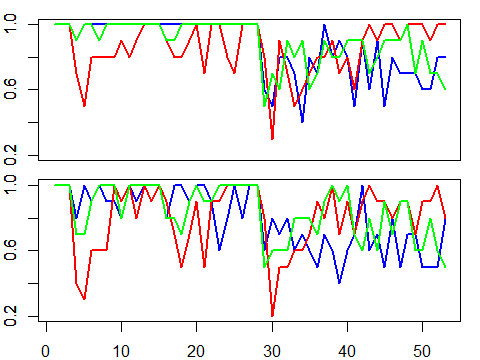
\includegraphics[width=0.9\columnwidth]{fig/acc_forg.png}}
\caption{Acurácia encontrada variando-se o fator de esquecimento. Acima os resultados do \textit{grid} e abaixo do \textit{quadtree}. A linha azul corresponde a um fator de 1/4, verde de 2/3 e vermelho de 9/10.}
\label{accforg}
\end{figure}

\begin{figure}[h]
\centerline{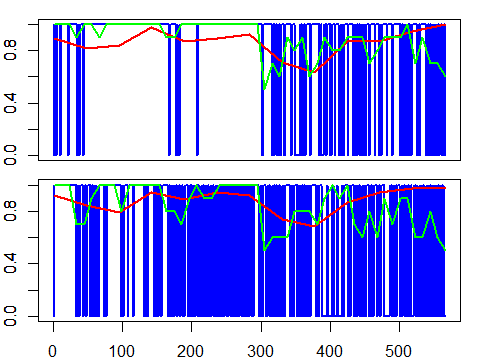
\includegraphics[width=0.9\columnwidth]{fig/acc_batch.png}}
\caption{Acurácia encontrada variando-se o tamanho dos pacotes. Acima os resultados do \textit{grid} e abaixo do \textit{quadtree}. A linha azul corresponde a um tamanho de 3, verde de 32 e vermelho de 128.}
\label{accbatch}
\end{figure}

\begin{figure}[h]
\centerline{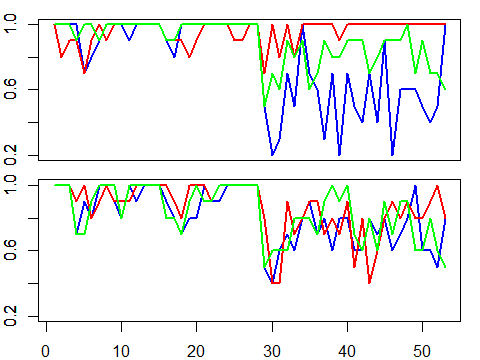
\includegraphics[width=0.9\columnwidth]{fig/acc_parts.png}}
\caption{Acurácia encontrada variando-se o número de divisões do espaço. Acima os resultados do \textit{grid} e abaixo do \textit{quadtree}. A linha azul corresponde a um grid e a um tamanho de árvore respectivamente de 8 e 4, verde de 16 e 5 e vermelho de 32 e 6.}
\label{accparts}
\end{figure}

\begin{figure}[h]
\centerline{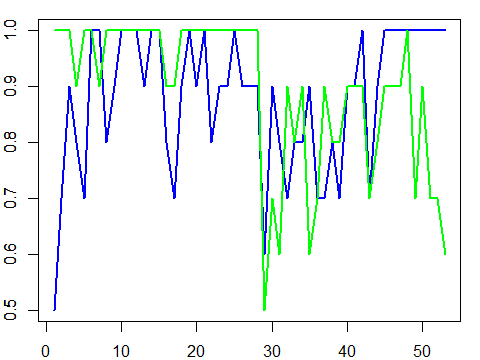
\includegraphics[width=0.9\columnwidth]{fig/acc_filt.png}}
\caption{Acurácia encontrada utilizando e não utilizando a filtragem no método do \textit{grid}. A linha em azul corresponde ao resultado sem a filtragem e em verde utilizando a filtragem.}
\label{accfilt}
\end{figure}

\begin{figure}[h]
\centerline{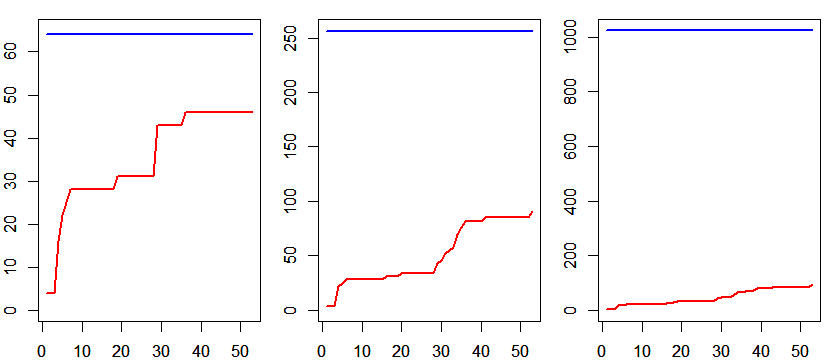
\includegraphics[width=0.9\columnwidth]{fig/mem_parts.png}}
\caption{Quantidade de elementos utilizados pelos métodos variando-se o número de divisões do espaço. Em azul para o \textit{grid} (correspondente ao tamanho máximo) e vermelho para o \textit{quadtree}. Da esquerda para a direita os valores utilizados de grid e tamanho de árvore foram respectivamente iguais a 8 e 4, 16 e 5 e 32 e 6.}
\label{memparts}
\end{figure}

\begin{figure}[h]
\centerline{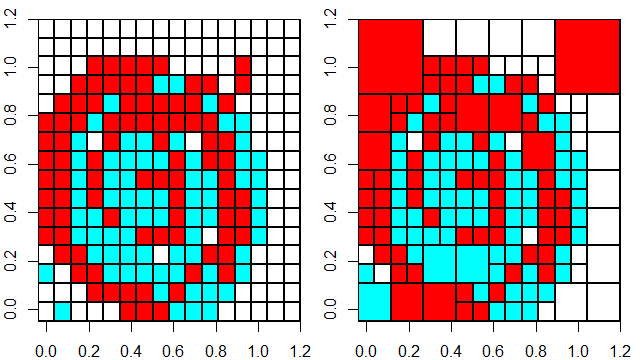
\includegraphics[width=0.7\columnwidth]{fig/off.png}}
\caption{Diferença observada entre o método do \textit{grid} sem a realização da filtragem (à esquerda) e do \textit{quadtree} (à direita).}
\label{off}
\end{figure}

\begin{figure}[h]
\centerline{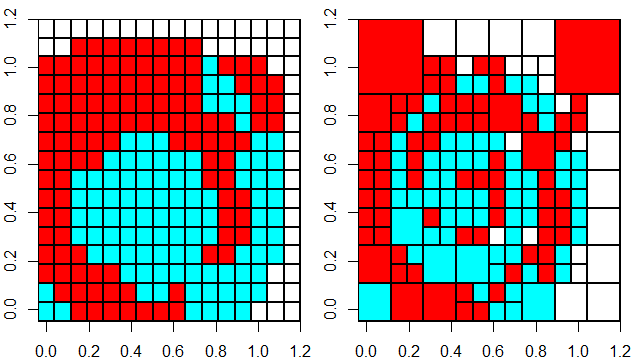
\includegraphics[width=0.7\columnwidth]{fig/off_filt.png}}
\caption{Diferença observada entre o método do \textit{grid} com a realização da filtragem (à esquerda) e do \textit{quadtree} (à direita).}
\label{offfilt}
\end{figure}

\begin{figure}[h]
\centerline{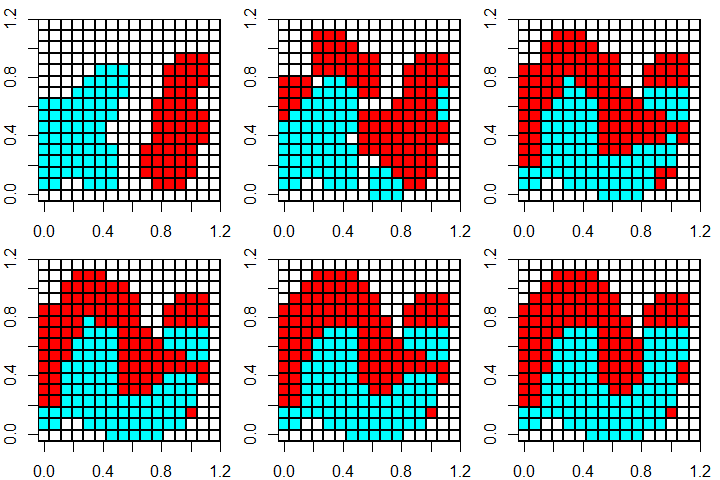
\includegraphics[width=1\columnwidth]{fig/drift_gmodel.png}}
\caption{Variação do modelo do \textit{grid} para a ocorrência de uma mudança de conceito. A ordem temporal é primeiro da esquerda para a direta e em seguida de cima para baixo.}
\label{driftgmodel}
\end{figure}

\begin{figure}[h]
\centerline{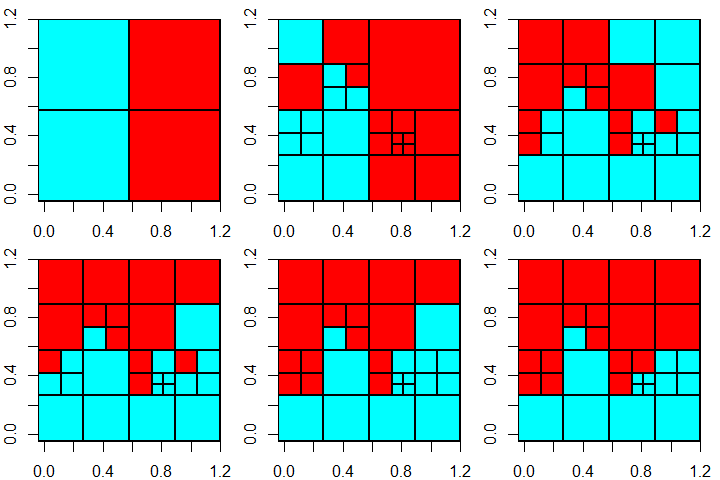
\includegraphics[width=1\columnwidth]{fig/drift_tmodel.png}}
\caption{Variação do modelo do \textit{quadtree} para a ocorrência de uma mudança de conceito. A ordem temporal é primeiro da esquerda para a direta e em seguida de cima para baixo.}
\label{drifttmodel}
\end{figure}

\begin{figure}[h]
\centerline{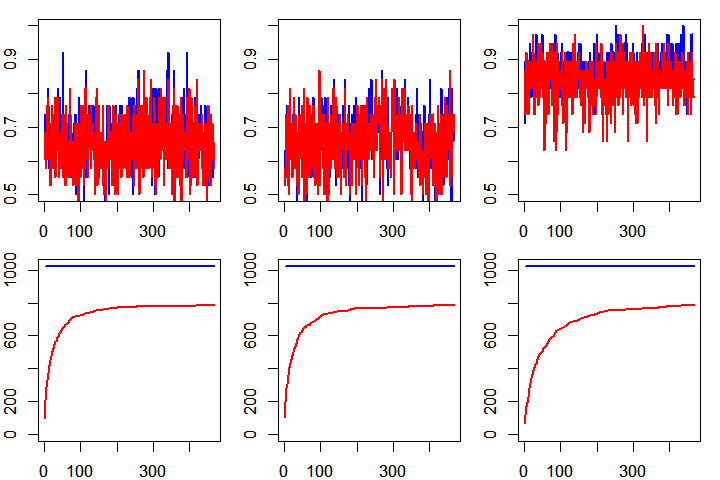
\includegraphics[width=1\columnwidth]{fig/sea_acc.png}}
\caption{Acima está representada a acurácia encontrada e abaixo a quantidade de elementos utilizados pelos métodos na base de dados \textit{fourclass}. Em azul para o \textit{grid} e vermelho para o \textit{quadtree}. Da direita para a esquerda  estão representadas as variáveis 1 e 2, 1 e 3, 2 e 3.}
\label{seaacc}
\end{figure}

\begin{figure}[h]
\centerline{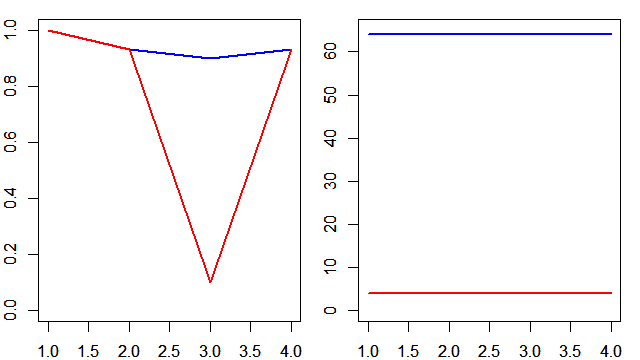
\includegraphics[width=0.9\columnwidth]{fig/four_acc.png}}
\caption{Acurácia encontrada (acima) e quantidade de elementos utilizados (abaixo) pelos métodos na base de dados \textit{fourclass}. Em azul para o \textit{grid} e vermelho para o \textit{quadtree}.}
\label{fouracc}
\end{figure}



\end{document}